\chapter{Estado del arte}
\label{ch:estado}
En este capítulo se presentan de una manera más detallada cuáles son los factores físicos que afectan a la seguridad de los CPD en la actualidad. Después se estudiarán y expondrán cuáles son las alternativas que existen actualmente que hacen algo parecido a lo que pretendemos desarrollar, lo que nos dará una visión general de la situación para desarrollar nuestro sistema. Por último, se analizarán las distintas alternativas de software y hardware para el sistema, escogiendo las que mejor se adapten al mismo.

\section{Seguridad física en los CPD}\label{sec:seguridad_fisica_CPD}
Según los criterios del Instituto Nacional de Ciberseguridad de España (INCIBE) para construir un CPD seguro es necesario tener en cuenta las siguientes áreas~\cite{noauthor_pon_2015}:
\begin{itemize}
	\item \textbf{Control de acceso:} Es uno de los aspectos de seguridad más importantes a tener en cuenta, porque nos permite evitar que personas ajenas puedan acceder a estos recintos y hagan un uso indebido de las instalaciones o provoque daños intencionadamente, del mismo modo, se tiene controlado al personal autorizado que pueda entrar en el recinto con intención de perjudicar a la empresa, manteniendo un registro de todos los accesos. Pueden instalarse sistema de acceso por huella digital, verificación de voz, lectores de tarjetas, etc.

	También se debe asegurar que no se pueda acceder a la sala mediante el empleo de la fuerza, con la instalación de puertas blindadas o acorazadas, o sistemas que eviten que las puertas puedan quedar abiertas accidentalmente, mediante el uso de sistemas de alarma si esto ocurre.
	\item \textbf{Seguimiento dentro de la sala:} Como complemento a lo anterior, es conveniente tener conocimiento de todo lo que haga el personal autorizado en el interior de estos recintos en cada momento. Esto se consigue con la instalación de equipos de videovigilancia o un circuito cerrado de televisión (CCTV).
	\item \textbf{Dificultar la identificación del CPD:} Dentro de lo posible es conveniente que el menor número de personas posible tenga conocimiento de la ubicación exacta del CPD, para evitar cualquier manipulación.
	\item \textbf{Medidas contra incendios:} Aparte de estar construidos con materiales resistentes a altas temperaturas o ignífugos, existirán sensores de humo y calor que permiten detectar si se está produciendo un incendio. En cuanto se detecte un incendio, se activará el sistema de extinción por gas, para evitar dañar los equipos. Estos sistemas pasarán revisiones periódicamente para su correcto funcionamiento.
	      \pagebreak
	\item \textbf{Seguridad del cableado:} Se emplea cableado apantallado para evitar acoplamientos o interferencias, además de estar claramente diferenciados según su función, como los de alimentación y de comunicaciones, para facilitar el mantenimiento del CPD\@.
	\item \textbf{Medidas contra problemas de suministro eléctrico:} Es otro de los sistemas fundamentales en los CPD, que permite mantener el suministro eléctrico necesario para garantizar la disponibilidad del servicio y evitar la pérdida o dañado de los datos y de los propios equipos. Las medidas que se toman a este respecto son la implantación de mecanismos de redundancia eléctrica para que los servidores no pierdan la alimentación eléctrica en caso de un corte de la empresa suministradora, como son los Sistemas de Alimentación Ininterrumpida (SAI) o grupos electrógenos.
	\item \textbf{Suelo y techo técnico:} Este tipo de suelos nos permiten, a la vez que elevar los equipos respecto al nivel original de la sala, distribuir todo el cableado necesario por debajo de él, siendo más fácil el mantenimiento, quedando la sala más limpia y despejada y garantizando una ventilación que evite sobrecalentamientos. El techo técnico permite lo mismo que el suelo, pero con las instalaciones por encima de un falso techo registrable permitiendo a la vez instalar el propio sistema de climatización de la sala. Ambos sistemas son muy importantes para el reducir el consumo de energía empleado para climatizar, hasta en un 45 \%~\cite{noauthor_suelo_2020}, además de permitir un constante movimiento del flujo de aire por la sala. Otra función que ofrecen es evitar los daños por inundación.
	\item \textbf{Sistema de climatización:} Se encarga de controlar la temperatura y humedad de la sala regulando el enfriamiento, ventilación, humidificación y flujo de aire. También existen sistemas que mantienen la temperatura idónea de los equipos mediante refrigeración líquida e incluso inmersos en fluidos dieléctricos.
	
	Además, hay sistemas que controlan la calidad del aire y la existencia de gases. Los límites ambientales recomendados internacionalmente son: para la temperatura, entre 18 °C y 27 °C, y para la humedad, entre el 40 \% y el 60 \%~\cite{noauthor_recommended_nodate}.
\end{itemize}

\iffalse
\section{Soluciones actuales}\label{sec:soluciones-actuales}
En esta sección se presentarán cuáles son las alternativas que existen actualmente y que tienen el mismo propósito que el sistema que se va a desarrollar en este proyecto.

Como se trata de un sistema de control ambiental y videovigilancia no cubriremos todos los aspectos de seguridad que se han presentado en la \autoref{sec:seguridad_fisica_CPD}, pero sí se desarrollaran: Seguimiento dentro de la sala, Medidas contra incendios y Sistema de climatización.

INCOMPLETO, FALTA ENCONTRARLAS

\section{Critica al Estado del arte}\label{sec:critica-al-estado-del-arte}
PUNTOS FUERTES DE CADA UNA
\fi

\section{Propuesta}\label{sec:propuesta}
El sistema que se va a desarrollar consistirá en un dispositivo de reducidas dimensiones que dispondrá de una placa y una serie de sensores, que tomaran los datos periódicamente y los enviaran a una base de datos que podrá ser consultada mediante una web.

Este dispositivo constará de las siguientes funcionalidades:
\begin{itemize}
	\item Proporcionar imagen en tiempo real del interior de la sala, que nos permitirá ver lo que ocurre y poder actuar de una manera eficaz ante cualquier circunstancia adversa que lo requiera. La imagen podrá ser vista, aparte de por el personal de seguridad si es que existe en el propio edificio, también por vía IP por la persona o personas encargadas de la misma mediante la clave necesaria.
	\item Controlar la temperatura y humedad ambiental de la sala, para detectar posibles fallos en el sistema de climatización o fugas de agua de instalaciones próximas que puedan provocar la entrada de agua en el recinto.
	\item Detección de incendios mediante el control del nivel de CO y CO$_2$, incluso antes de que pueda llegar a producirse llama, como en el caso de una combustión inicial e incompleta de algunos materiales, que emitirían CO o cuando se haya llegado a producir esta, con la emisión de CO$_2$.
	\item Control de la calidad del aire del recinto, para evitar el deterioro precoz de algunos equipos sensibles a las partículas en suspensión.
\end{itemize}

\section{Estudio de Alternativas de Solución}\label{sec:estudio-de-alternativas-de-solución}
En esta sección se presentarán las distintas alternativas que se pueden utilizar para dar solución a cada una de las necesidades planteadas en la \autoref{sec:propuesta}.

\subsection{Alternativas: Placa}\label{subsec:altPlacas}
Para comenzar debemos analizar cuáles son las posibles placas sobre las que podemos desarrollar nuestro dispositivo. Las placas que se buscan deben ser programables y permitirnos instalar una serie de sensores que podamos monitorear, por esta razón se ha decidido evaluar la línea de productos de Raspberry Pi Foundation. 

\begin{figure}[H]
	\ffigbox[\FBwidth]
	{\caption{Logo Raspberry Pi}}
	{\def\svgwidth{.21\textwidth}
		\input{./imagenes/Raspberry_Pi_Logo.eps_tex}}\label{fig:logoRaspberry}
\end{figure}

Raspberry Pi es una computadora de una sola placa (SBC) de bajo coste, que comenzaron a venderse en 2012 y son las ideales para proyectos de electrónica que requieran de una máquina potente de reducidas de dimensiones. Cuenta con su propio sistema operativo y es capaz de funcionar como un ordenador completo. Todas las versiones incluyen un procesador Broadcom, RAM, GPU, conexión de cámara y 40 pines GPIO (Entrada/Salida de Propósito General), pero no cuentan con memoria interna y debe ser añadida por MicroSD~\cite{noauthor_raspberry_2021}.

A continuación se presentan las valoradas para este proyecto, que son el modelo reducido para domótica y los dos modelos más recientes~\cite{noauthor_raspberry_nodate}:
\begin{figure}[!htb]
	\minipage{0.32\textwidth}
	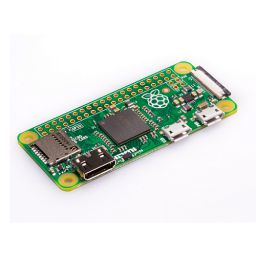
\includegraphics[width=\linewidth]{raspberry-pi-zero.jpg}
	\caption{Raspberry Pi Zero, Raspberry Pi 3 B+ y Raspberry Pi 4 B}
	\endminipage\hfill
	\minipage{0.32\textwidth}
	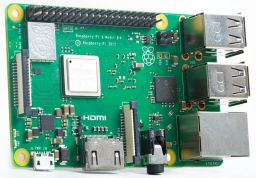
\includegraphics[width=\linewidth]{raspberry-pi-3b-plus.jpg}
	\endminipage\hfill
	\minipage{0.32\textwidth}%
	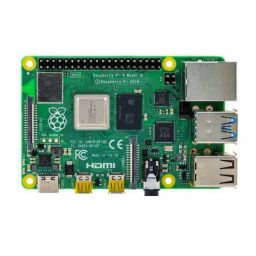
\includegraphics[width=\linewidth]{raspberry-pi-4-b.jpg}
	\endminipage\label{fig:fotosRaspberry}
\end{figure}
\begin{table}[H]
	\centering
	\caption{Comparación gama Raspberry Pi}
	\label{tab:comp_placas}
	\resizebox{\textwidth}{!}{%
		\begin{tabular}{|l|c|c|c|}
			\hline
			                                     & \cellcolor[HTML]{BFBFBF}\textbf{Raspberry Pi Zero} & \cellcolor[HTML]{BFBFBF}\textbf{Raspberry Pi 3 B+} & \cellcolor[HTML]{BFBFBF}\textbf{Raspberry Pi 4 B} \\ \hline
			\cellcolor[HTML]{BFBFBF}CPU          & \begin{tabular}[c]{@{}c@{}}1-GHz, 1-core\\ Broadcom BCM2835\\ (ARM1176JZF-S)\end{tabular}                          & \begin{tabular}[c]{@{}c@{}}1.4-GHz, 4-core\\ Broadcom BCM2837B0\\ (Cortex-A53)\end{tabular}                          & \begin{tabular}[c]{@{}c@{}}1.5-GHz, 4-core\\ Broadcom BCM2711\\ (Cortex-A72)\end{tabular}                         \\ \hline
			\cellcolor[HTML]{BFBFBF}RAM          & \begin{tabular}[c]{@{}c@{}}LPDDR2\\ 512 MB\end{tabular}                          & \begin{tabular}[c]{@{}c@{}}LPDDR2\\ 1 GB\end{tabular}                          & \begin{tabular}[c]{@{}c@{}}LPDDR4\\ 1, 2, 4 GB\end{tabular}                        \\ \hline
			\cellcolor[HTML]{BFBFBF}USB          & 1 Micro                                            & 4 (2.0)                                            & \begin{tabular}[c]{@{}c@{}}2 (2.0)\\ 4 (3.0)\end{tabular}                        \\ \hline
			\cellcolor[HTML]{BFBFBF}Alimentación & microUSB                                           & microUSB                                           & USB Tipo-C                                        \\ \hline
			\cellcolor[HTML]{BFBFBF}HDMI         & MiniHDMI                                           & HDMI                                               & 2 Micro HDMI                                      \\ \hline
			\cellcolor[HTML]{BFBFBF}Ethernet     & No                                                 & Gigabit 300 Mbps                                   & True Gigabit                                      \\ \hline
			\cellcolor[HTML]{BFBFBF}Wi-Fi        & No                                                 & Dual-band Wi-Fi                                    & Dual-band Wi-Fi                                   \\ \hline
			\cellcolor[HTML]{BFBFBF}Bluetooth    & No                                                 & 4.2                                                & 5.0                                               \\ \hline
			\cellcolor[HTML]{BFBFBF}Tamaño       & 65 x 30 mm                                         & 85 x 30 mm                                         & 85 x 30 mm                                        \\ \hline
			\cellcolor[HTML]{BFBFBF}Precio       & 5,4 euros                                          & 39 euros                                           & 39, 61 o 93 euros                                 \\ \hline
		\end{tabular}%
	}
\end{table}

\subsection{Alternativas: Componentes}\label{subsec:altComponentes}
Se estudiarán los diferentes sensores y cámaras que se podrán integrar en el dispositivo, para controlar el estado y ambiente de la sala con la finalidad de mantener la seguridad de los equipos que se encuentra en la misma.

\paragraph{Sensores}\mbox{} \\
Como se explicó en la propuesta se han buscado sensores capaces de captar temperatura, humedad, CO, CO$_2$ y la calidad del aire. A continuación se exponen los sensores que se han encontrado y que cubren estas necesidades. Más adelante decidiremos si se adaptan al proyecto.

Comencemos con el sensor de temperatura y humedad, que es frecuente que ambos aparezcan juntos en el mismo sensor~\cite{noauthor_comparing_2019}:

\begin{table}[H]
	\centering
	\caption{Comparación sensores de temperatura y humedad}
	\label{tab:comp_temp}
	\resizebox{\textwidth}{!}{%
		\begin{tabular}{|l|c|c|c|c|c|c|}
			\hline
			                                                   & \cellcolor[HTML]{BFBFBF}\textbf{DHT11}                 & \cellcolor[HTML]{BFBFBF}\textbf{DHT22} & \cellcolor[HTML]{BFBFBF}\textbf{LM35} & \cellcolor[HTML]{BFBFBF}{\color[HTML]{3A3A3A} \textbf{DS18B20}} & \cellcolor[HTML]{BFBFBF}{\color[HTML]{3A3A3A} \textbf{BME280}} & \cellcolor[HTML]{BFBFBF}{\color[HTML]{3A3A3A} \textbf{BMP180}} \\ \hline
			\cellcolor[HTML]{BFBFBF}Temperatura                & Si                                                     & Si                                     & Si                                    & Si                                                              & Si                                                             & Si                                                             \\ \hline
			\cellcolor[HTML]{BFBFBF}Humedad                    & Si                                                     & Si                                     & No                                    & No                                                              & Si                                                             & No                                                             \\ \hline
			\cellcolor[HTML]{BFBFBF}\begin{tabular}[c]{@{}l@{}}Protocolo de\\ comunicación\end{tabular} & 1 cable                                                & 1 cable                                & Analógico                             & 1 cable                                                         & I2C                                                            & I2C                                                            \\ \hline
			\cellcolor[HTML]{BFBFBF}Voltaje                    & 3 -- 5.5 V                                              & 3 -- 6 V                                & 4 -- 30 V                              & 3 -- 5.5 V                                                       & \begin{tabular}[c]{@{}c@{}}1.7 -- 3.6 V chip\\ 3.3 -- 5 V placa\end{tabular}                                     & \begin{tabular}[c]{@{}c@{}}1.8 -- 3.6 V chip\\ 3.3 -- 5 V placa\end{tabular}                                     \\ \hline
			\cellcolor[HTML]{BFBFBF}\begin{tabular}[c]{@{}l@{}}Rango de\\ temperatura\end{tabular} & 0 -- 50ºC                                               & -40 -- 80ºC                             & -55 -- 150ºC                           & -55 -- 125ºC                                                     & -40 -- 85ºC                                                     & 0 -- 65ºC                                                       \\ \hline
			\cellcolor[HTML]{BFBFBF}\begin{tabular}[c]{@{}l@{}}Precisión de\\ temperatura\end{tabular} & \cellcolor[HTML]{FFFFFF}{\color[HTML]{3A3A3A} +/- 2ºC} & +/- 0.5ºC                              & +/-0.5ºC                              & +/-0.5ºC                                                        & +/-0.5ºC                                                       & +/-0.5ºC                                                       \\ \hline
			\cellcolor[HTML]{BFBFBF}\begin{tabular}[c]{@{}l@{}}Rango de\\ humedad\end{tabular} & 20 -- 80\%                                                & 0 -- 100\%                                & -                                     & --                                                               & 0 -- 100\%                                                        & -                                                              \\ \hline
			\cellcolor[HTML]{BFBFBF}\begin{tabular}[c]{@{}l@{}}Precisión de\\ humedad\end{tabular} & +/- 5\%                                                & +/- 2-5\%                              & -                                     & -                                                               & +/- 4\%                                                        & -                                                              \\ \hline
			\cellcolor[HTML]{BFBFBF}Precio                     & 6,99 euros                                             & 10,99 euros                            & 6,07 euros                            & 0.82 euros                                                      & 7,23 euros                                                     & 2,02 euros                                                     \\ \hline
		\end{tabular}%
	}
\end{table}

Para el sensor de monóxido de carbono (CO) no se encontraron muchas posibilidades, por lo que se ha optado por el MQ7, cuyas especificaciones son las siguientes.
\vspace{-2cm}
\minipage{0.4\textwidth}
\begin{figure}[H]
	\caption{Sensor MQ-7}
	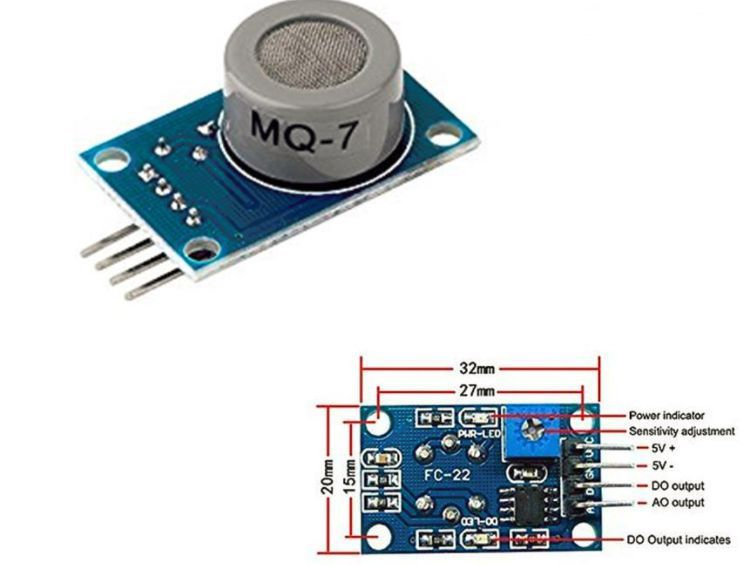
\includegraphics[width=\linewidth]{mq7.jpg}\label{fig:sensorMQ-7}
\end{figure}
\endminipage\hfill
\minipage{0.5\textwidth}
\begin{table}[H]
	\centering
	\caption{Especificaciones módulo MQ-7}
	\label{tab:mq_7}
	\begin{tabular}{|
		>{\columncolor[HTML]{BFBFBF}}l |l|}
		\hline
		\textbf{Alimentación}               & 5 V                        \\ \hline
		\textbf{Intensidad}                 & 140 m                      \\ \hline
		\textbf{Tipo}                       & Analógico                  \\ \hline
		\textbf{Precalentamiento}           & 20 s                       \\ \hline
		\textbf{\begin{tabular}[c]{@{}l@{}}Tiempo de\\ respuesta\end{tabular}} & 1 ms                       \\ \hline
		\textbf{Pines}                      & \begin{tabular}[c]{@{}l@{}}GND\\ DOUT\\ AOUT\\ VCC\end{tabular} \\ \hline
		\textbf{Rango}                      & 10 -- 10.000 ppm             \\ \hline
		\textbf{Tamaño}                     & 40x20 mm                   \\ \hline
	\end{tabular}
\end{table}
\endminipage

A continuación se muestran los sensores de dióxido de carbono (CO$_2$) que se han considerado para este proyecto.

\begin{table}[H]
	\centering
	\caption{Comparación sensores CO$_2$}
	\label{tab:comp_co2}
	\resizebox{\textwidth}{!}{%
		\begin{tabular}{|l|c|c|c|c|}
			\hline
			                                                   & \cellcolor[HTML]{BFBFBF}\textbf{MH-Z14A} & \cellcolor[HTML]{BFBFBF}\textbf{CCS811} & \cellcolor[HTML]{BFBFBF}\textbf{S8 LP} & \cellcolor[HTML]{BFBFBF}\textbf{MG-811} \\ \hline
			\cellcolor[HTML]{BFBFBF}Voltaje                    & 4.5 -- 5,5 V                              & 3,3 -- 5 V                               & 4.5 -- 5,25 V                           & 5 V                                     \\ \hline
			\cellcolor[HTML]{BFBFBF}Rango                      & 0 -- 10.000 ppm                           & 400 -- 29.206 ppm                        & 400 -- 2.000 ppm                        & 0 -- 10.000 ppm                          \\ \hline
			\cellcolor[HTML]{BFBFBF}\begin{tabular}[c]{@{}l@{}}Protocolo de\\ comunicación\end{tabular} & UART                                     & I2C                                     & UART                                   & Analógico                               \\ \hline
		\end{tabular}%
	}
\end{table}
\vspace{-.7cm}

Por último, antes de pasar a la parte de videovigilancia, se muestran las especificaciones del módulo de calidad de aire que se ha considerado más adecuado. En este caso no se muestran varias posibilidades dada la escasa variedad de módulos que solo incorporen este tipo de sensor. Todos los encontrados eran parte de sistemas mucho más complejos que eran capaces de funcionar de manera independiente. Se ha escogido el módulo SDS011 que es capaz de medir las partículas en suspensión (PM) de 2,5 y 10 micrómetros, cuyas características son las siguientes~\cite{noauthor_nova_nodate}:
\vspace{-1cm}

\minipage{0.45\textwidth}
\begin{figure}[H]
	\caption{Sensor SDS011}
	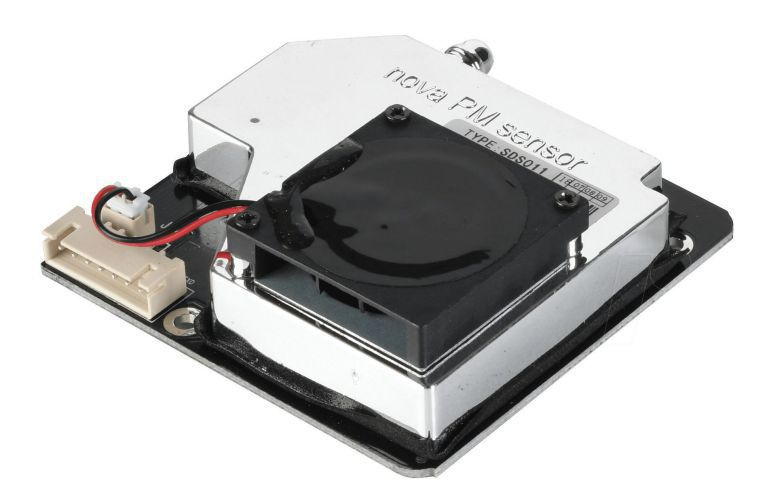
\includegraphics[width=\linewidth]{SDS011.jpg}\label{fig:sds011}
\end{figure}
\endminipage\hfill
\minipage{0.45\textwidth}
\begin{table}[H]
	\centering
	\caption{Especificaciones módulo SDS011}
	\label{tab:sds011}
	\resizebox{\linewidth}{!}{%
		\begin{tabular}{|
			>{\columncolor[HTML]{BFBFBF}}l |l|}
			\hline
			\textbf{Voltaje}             & 5 V                                                        \\ \hline
			\textbf{Corriente máxima}    & 100 mA                                                     \\ \hline
			\textbf{Rango}               & 0 -- 999.9 ug/m3                                            \\ \hline
			\textbf{Resolución}          & 0,3 ug/m3                                                  \\ \hline
			\textbf{Error relativo}      & 10 \%                                                      \\ \hline
			\textbf{Tiempo de respuesta} & 1 s                                                        \\ \hline
			\textbf{Salida}              & UART (USB)                                                 \\ \hline
			\textbf{Tamaño}              & 71x70x23 mm \\ \hline
		\end{tabular}%
	}
\end{table}
\endminipage

\paragraph{Cámaras}\mbox{} \\
Las cámaras que se presentan a continuación han sido buscadas con la intención de que sean compatibles con la Raspberry Pi, por lo que su conexión debe ser mediante la CSI de la placa. Se han propuesto una serie de cámaras con diferentes categorías~\cite{cholewiak_raspberry_2017}, algunas cuentan con una mejor resolución, angular o ambos. Aun así las cuatro cámaras tienen los mismos modos de grabación: 1080p30, 720p60 y 640×480p60/90.

\begin{table}[H]
	\centering
	\caption{Comparación de módulos cámara}
	\label{tab:comp_camara}
	\resizebox{\textwidth}{!}{%
		\begin{tabular}{|l|c|c|c|c|}
			\hline
			                                                   & \cellcolor[HTML]{BFBFBF}\textbf{\begin{tabular}[c]{@{}c@{}}Raspberry Pi\\ Camera\end{tabular}}        & \cellcolor[HTML]{BFBFBF}\textbf{\begin{tabular}[c]{@{}c@{}}Raspberry Pi v2\\ Camera\end{tabular}} & \cellcolor[HTML]{BFBFBF}\textbf{\begin{tabular}[c]{@{}c@{}}Waveshare RPi\\ Camera (I)\end{tabular}}        & \cellcolor[HTML]{BFBFBF}\textbf{Sony IMX477}                       \\ \hline
			\cellcolor[HTML]{BFBFBF}Megapíxeles                & 5                                                                  & 8                                                           & 5                                                                  & 12.3                                                               \\ \hline
			\cellcolor[HTML]{BFBFBF}FOV                        & 54°                                                                & 62.2°                                                       & 170°                                                               & Depende de la lente                                                \\ \hline
			\cellcolor[HTML]{BFBFBF}\begin{tabular}[c]{@{}l@{}}Resolución\\ del sensor\end{tabular} & \cellcolor[HTML]{FFFFFF}{\color[HTML]{2A2A2A} 2592 × 1944 pixeles} & 3280 × 2464 pixeles                                         & \cellcolor[HTML]{FFFFFF}{\color[HTML]{2A2A2A} 2592 × 1944 pixeles} & \cellcolor[HTML]{FFFFFF}{\color[HTML]{2A2A2A} 4056 x 3040 pixeles} \\ \hline
			\cellcolor[HTML]{BFBFBF}Precio                     & 19,70 euros                                                        & 24,95 euros                                                 & 28,01 euros                                                        & 50 euros                                                           \\ \hline
		\end{tabular}%
	}
\end{table}

\section{Hardware y Software seleccionado}\label{sec:hardwareSoftware}
En esta sección se escogerá una solución de entre las expuestas en las subsecciones antes descritas.

\subsection{Placa}\label{subsec:placa}
Entre las tres placas que se han valorado, aunque la Zero está más pensada para dispositivos ligeros y compactos, se ha decidido descartarla por sus reducidas capacidades y la falta de wifi o ethernet que requerirían un módulo extra para obtener conexión a internet. Entre las dos restantes se ha optado por la Raspberry Pi 3B+, porque ante la similitud de características de las placas y su coste, esta tenía más disponibilidad en el mercado y el suministro era más rápido. 
\begin{figure}[H]
	\ffigbox[\FBwidth]
	{\caption{Esquema de Raspberry Pi 3 B+}}
	{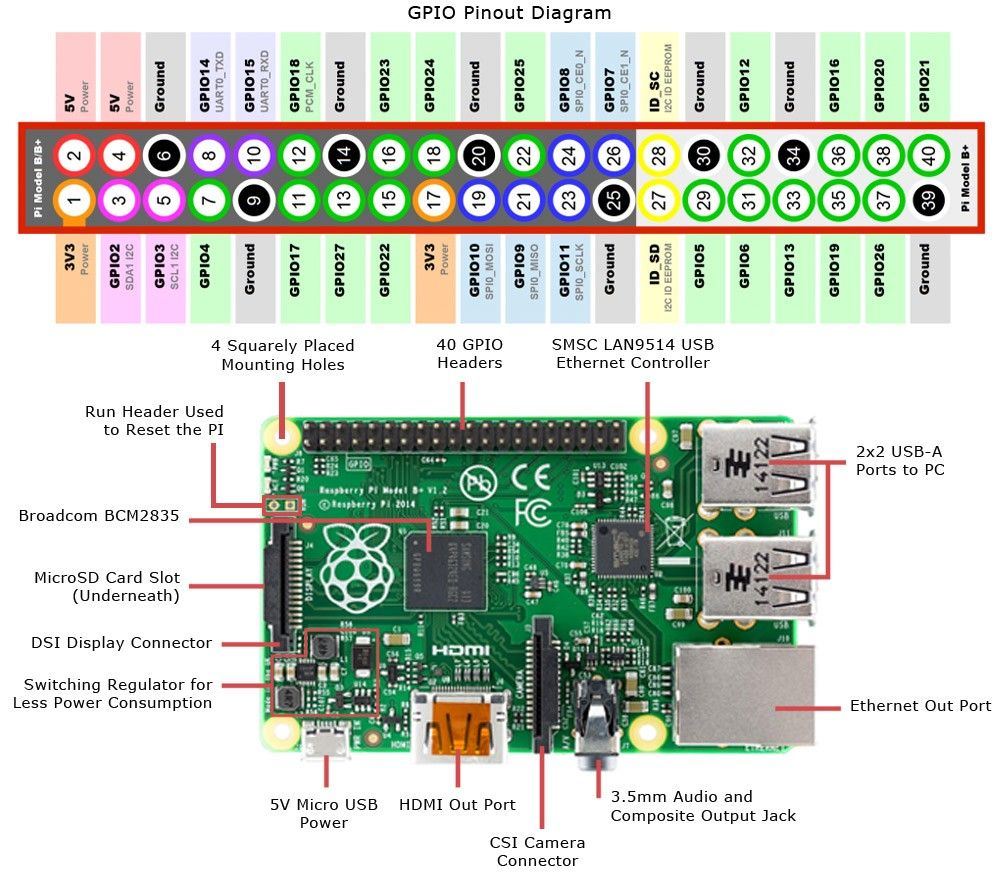
\includegraphics[scale=0.35]{esquema-raspberry-pi-3b-plus.jpg}}\label{fig:esquemaRaspberry3B}
\end{figure}
En cuanto al sistema operativo que se emplea en esta placa, se ha decidido utilizar Raspbian que es una distribución de Linux basado en Debian que está altamente optimizada para estas placas, además por tratarse de un sistema operativo que es conocido por el programador que llevara a cabo el desarrollo.

\subsection{Componentes}\label{subsec:componentes}
El sensor de temperatura y humedad que se ha elegido como la mejor opción ha sido el DHT11. Por un precio reducido es capaz de medir tanto temperatura como humedad, ambas en el rango en el que se mueven las medidas en un CPD (18 °C -- 27 °C y  40 \% -- 60 \%) con una precisión aceptable. La decisión por el DHT11 y no el DHT22 ha sido que tiene un mayor coste y supera, con mucho, las temperaturas que se medirían, desaprovechando sus capacidades.
\begin{figure}[H]
	\ffigbox[\FBwidth]
	{\caption{Sensor DHT11}}
	{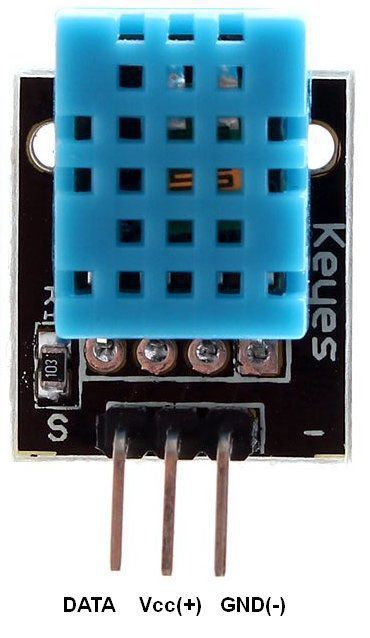
\includegraphics[scale=0.35]{dht11.jpg}}\label{fig:dht11}
\end{figure}
El sensor de CO$_2$ por el que nos hemos decantado ha sido el MH-Z14A, que ante unas capacidades similares al MG-811 se ha preferido el protocolo de comunicación UART. Por otro lado el CCS811 a pesar de tener muy buenas características su rango comienza demasiado arriba para captar la concentración atmosférica común, cosa que el MH-Z14A si capta y su cota más alta es suficiente para este proyecto.
\begin{figure}[H]
	\ffigbox[\FBwidth]
	{\caption{Sensor MH-Z14A}}
	{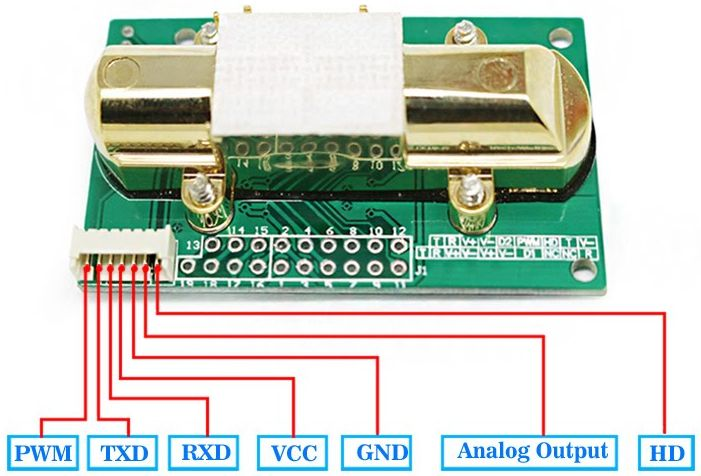
\includegraphics[scale=0.4]{MH-Z14A.jpg}}\label{fig:mh-z14a}
\end{figure}
Con respecto al sensor de CO y al de calidad el aire, se ha escogido el MQ-7 y SDS011 por la falta de variedad y disponibilidad en esta clase de sensores, pero esto no ha hecho que se hayan escogido componentes de peor calidad o que no vayan a desempeñar su función adecuadamente.

En cuanto a la cámara, tras analizar las especificaciones de las candidatas, se ha decidido que la que mejor se adapta al proyecto es la Raspberry Pi Camera. Se ha seleccionado esta cámara dado que todas ellas graban con las mismas resoluciones y frecuencias de cuadros, y como se trata de un dispositivo orientado a videovigilancia no buscamos que la resolución de las fotos sea la mejor, sino que pueda proporcionar una buena imagen a tiempo real por un bajo coste. Además el angular de la Raspberry Pi Camera es suficiente para captar lo que se encuentra dentro de la sala.
\begin{figure}[H]
	\ffigbox[\FBwidth]
	{\caption{Modulo Raspberry Pi Camera}}
	{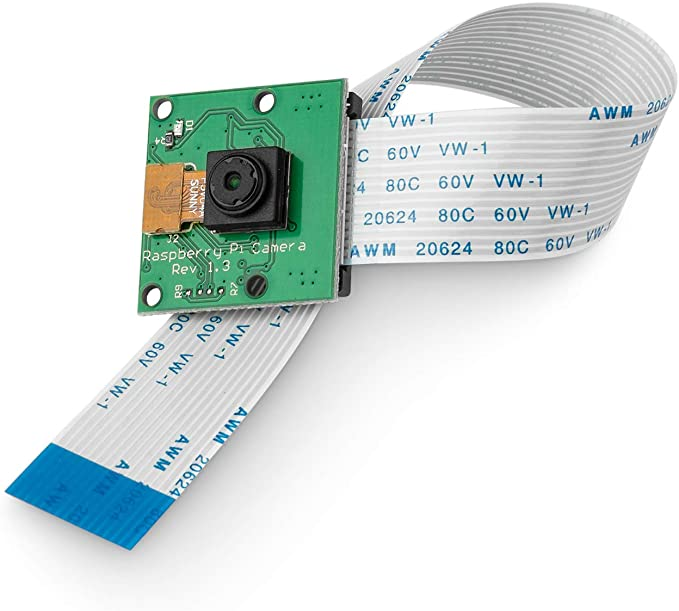
\includegraphics[scale=0.35]{Raspberry-Pi-Camera-Module-Rev-1.3.jpg}}\label{fig:moduloCamara}
\end{figure}

\subsection{Lenguajes de programación}\label{subsec:lenguajes}
En esta subsección se expondrán los lenguajes que se emplearán tanto para el desarrollo del dispositivo como para la parte web del proyecto. Los lenguajes han sido escogidos en función del conocimiento del programador que lo llevara a cabo, estos lenguajes son PHP para la web y Python para el dispositivo.
\pagebreak

\paragraph{PHP}\mbox{} \\
\begin{figure}[H]
	\ffigbox[\FBwidth]
	{\caption{Logo PHP}}
	{
\includegraphics[scale=0.08]{phplogo.jpg}}\label{fig:phpLogo}
\end{figure}
PHP (Hypertext Preprocessor)~\cite{welling_php_2003} es un lenguaje de programación para desarrollo web de código abierto desde el lado del servidor, creado originalmente en 1994 por Rasmus Lerdorf, aunque hoy en día es producido por The PHP Group. Este lenguaje puede ser embebido en una página HTML para que se ejecute cada vez que sea visualizado, el código en este lenguaje es interpretado por el servidor para convertirlo en otro lenguaje de salida.

Es el más utilizado en toda la red en abril de 2021~\cite{noauthor_usage_nodate} con un 79 \% de uso en los sitios web de los que se conoce el lenguaje del lado del servidor en 2021.

Para desarrollar la web se utilizará el editor de código fuente Visual Studio Code, editor multiplataforma de código abierto creado por Microsoft en 2015~\cite{noauthor_visual_2021} que dispone de infinidad de extensiones para facilitar el desarrollo en cualquier lenguaje de programación.

\paragraph{Python}\mbox{} \\
\begin{figure}[H]
	\ffigbox[\FBwidth]
	{\caption{Logo Python}}
	{
\includegraphics[scale=0.1]{Python-logo.jpg}}\label{fig:logoPython}
\end{figure}
Python es un lenguaje de programación de alto nivel interpretado desarrollado por la Python Software Foundation en 1991~\cite{montoro_python_2012}, cuya intención es facilitar la legibilidad del código haciendo la programación más accesible para todo el mundo. Su uso ha aumentado mucho en la última década llegando a ser uno de los lenguajes de propósito general más extendidos, puede ser utilizado para multitud de propósitos a diferencia de muchos otros lenguajes que se centran en un área específica.

Para programar todo el comportamiento del dispositivo se empleará este lenguaje por su sencillez y utilidad, el IDE que empleara el programador será PyCharm Professional edition creado por JetBrains en 2010~\cite{noauthor_pycharm_2021} al que se tiene acceso gracias a la licencia de estudiante, aunque también hay una edición gratuita llamada Community edition.

Se ha decidido el uso de este, en vez de emplear también Visual Studio Code, al estar orientado al desarrollo de programas en Python y por la posibilidad de conectarse vía SSH con la Raspberry Pi para sincronizar los programas y facilitar el proceso.

\subsection{Servidor y Base de datos}\label{subsec:servidorDB}
\begin{figure}[H]
	\ffigbox[\FBwidth]
	{\caption{Logo XAMPP}}
	{
\includegraphics[scale=0.13]{xampp.png}}\label{fig:logoXAMPP}
\end{figure}
El servidor que se va a emplear para este proyecto será Apache~\cite{noauthor_apache_nodate}, uno de los servidores de código abierto más utilizados que nos permite alojar y ser propietarios de nuestra propia web.

En cuanto a la base de datos utilizaremos MariaDB~\cite{noauthor_mariadb_nodate} que es un software de código abierto derivado y compatible con MySQL, que actualmente es de Oracle y de pago, pero mantiene la esencia de este gestor de base de datos.

Todo esto se orquestará mediante XAMPP una herramienta de software libre multiplataforma~\cite{noauthor_xampp_nodate} que nos permite crear el servidor y base de datos alojada por nosotros mismos. Este software nos ofrece desde un mismo sitio lanzar nuestra base de datos MariaDB, el servidor web Apache y los intérpretes de PHP y Perl.